\section{Setup Greenbone}
\sectionframe
\begin{frame}
    \frametitle{Debian}
    \begin{columns}
        \begin{column}{0.25\textwidth}
            \begin{itemize}
                \item Show the Debian VM
                \item Go to the VM's console
                \item Log in with the credentials \texttt{root:root}
            \end{itemize}
        \end{column}
        \begin{column}{0.75\textwidth}
            \begin{center}
                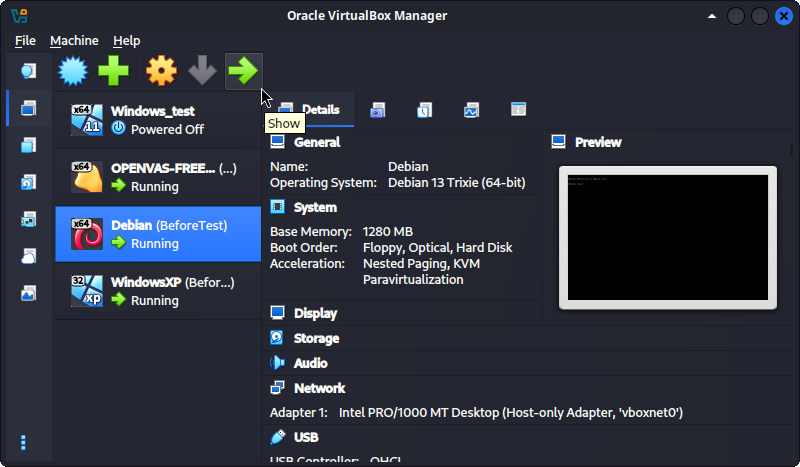
\includegraphics[width=1.0\textwidth]{images/debian_show.png}
            \end{center}
        \end{column}
    \end{columns}
\end{frame}

\begin{frame}
    \frametitle{Launch a bash script in Debian}
    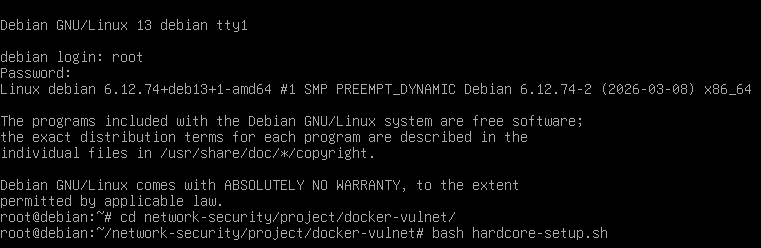
\includegraphics[width=1.0\textwidth]{images/debian_start.png}
    \texttt{cd network-security/project/docker-vulnet/}\\
    \texttt{bash hardcore-setup.sh}
\end{frame}

\begin{frame}[fragile]
    \frametitle{Check Debian IP Address}
    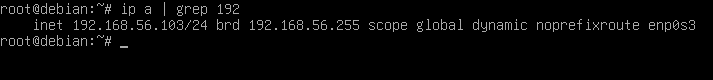
\includegraphics[width=1.0\textwidth]{images/debian_ip.png}
    \texttt{ip a | grep 192}\\
    It should output something like \texttt{192.160.56.10X}
\end{frame}

\begin{frame}[fragile]
    \frametitle{Set Greenbone Gateway}
    \begin{center}
        \begin{tabular}{cc}
            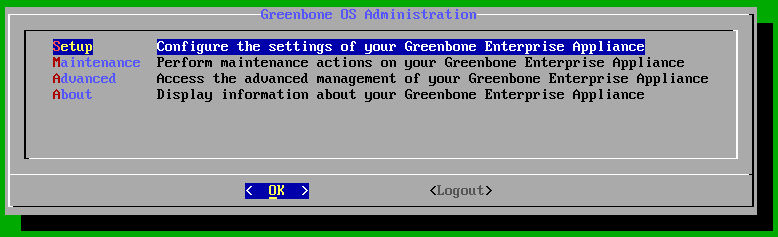
\includegraphics[width=0.47\textwidth]{images/gs_gateway_1.png} &
            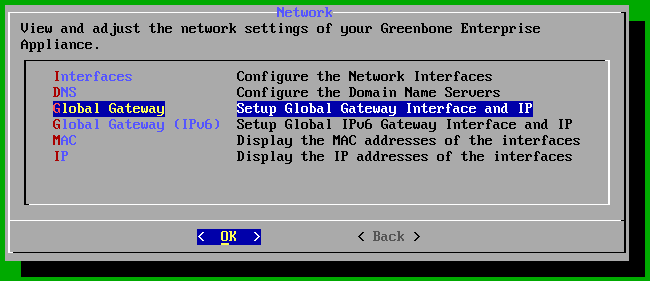
\includegraphics[width=0.47\textwidth]{images/gs_gateway_3.png} \\
            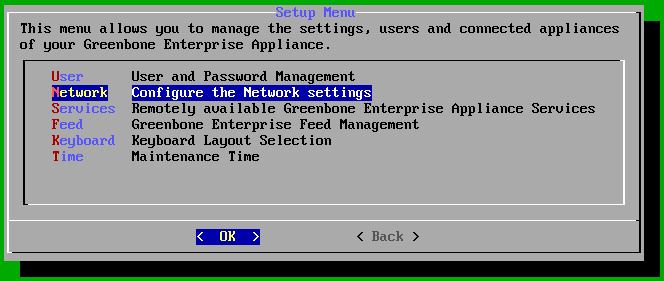
\includegraphics[width=0.47\textwidth]{images/gs_gateway_2.png} &
            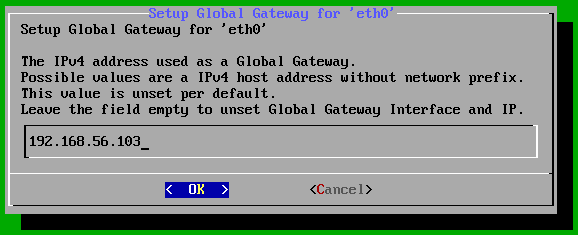
\includegraphics[width=0.47\textwidth]{images/gs_gateway_4.png}
        \end{tabular}
    \end{center}
\end{frame}

\begin{frame}[fragile]
    \frametitle{Remeber to save the settings}
    \begin{center}
        \begin{tabular}{cc}
            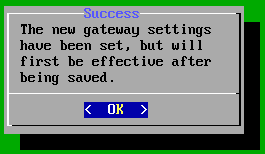
\includegraphics[height=0.375\textheight]{images/gs_gateway_5.png} &
            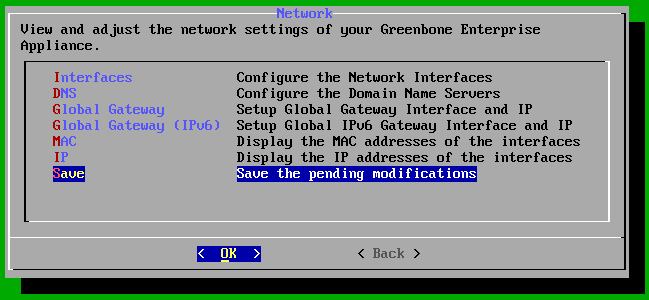
\includegraphics[height=0.375\textheight]{images/gs_gateway_6.png}
        \end{tabular}
    \end{center}
\end{frame}
